\documentclass[a4paper,11pt]{article}

\usepackage{graphicx}
\usepackage[margin=2.8cm]{geometry}
\usepackage{wrapfig}
\usepackage[colorlinks=true,urlcolor=blue,linkcolor=black]{hyperref}
\usepackage{color}
\usepackage[english]{babel}
\usepackage{forloop}

\newenvironment{reqlist}{\par \medskip \noindent \begin{tabular}{cp{0.83\textwidth}r} \\[-24pt]}{\end{tabular}}
\newcommand\req{\\ \smallskip \smallskip \hspace{0.24cm} $\bullet$\hspace{-0.2cm} & }

\newcounter{num}
\newcommand\effort[1]{\mbox{(\forloop{num}{0}{\value{num} < #1}{$\star$})}}
\newcommand{\quotes}[1]{``#1''}

\begin{document}
	
\thispagestyle{empty}

\noindent
\hrulefill \vspace{6pt}

\noindent

\includegraphics[viewport=8 8 185 55]{figures/eth_logo_black} \hfill

\includegraphics[trim=0 0 2 0]{figures/disco-logo-col} \hspace{-6pt} \vspace{-6pt}

\noindent \hrulefill \vspace{4pt}

\hfill Prof.\ R.\ Wattenhofer

\vspace{4pt}

\noindent \textbf{\LARGE Adaptive Hierarchical Deep Reinforcement Learning} \bigskip

\begin{wrapfigure}{l}{2.5cm}
	\vspace{-0.5cm}
	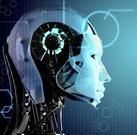
\includegraphics[width=2.5cm]{figures/robot}
\end{wrapfigure}

\noindent In 2015 Google Deepmind published their DQN paper in which they present an algorithm capable of learning to play Atari games at superhuman performance. Since then, research and applications of deep reinforcement learning (DRL) have gained more and more momentum. Results range from algorithms capable of mastering chess within 4 hours\footnote{\url{https://arxiv.org/abs/1712.01815}} to neural networks capable of constructing other neural networks.\footnote{\url{https://arxiv.org/abs/1611.01578}}

In this thesis we look into the abstracting the task time scale through hierarchical reinforcement learning and aim to develop an agent that is capable of addapting to new tasks.

\begin{wrapfigure}{r}{7.5cm}
	\vspace{-0.5cm}
	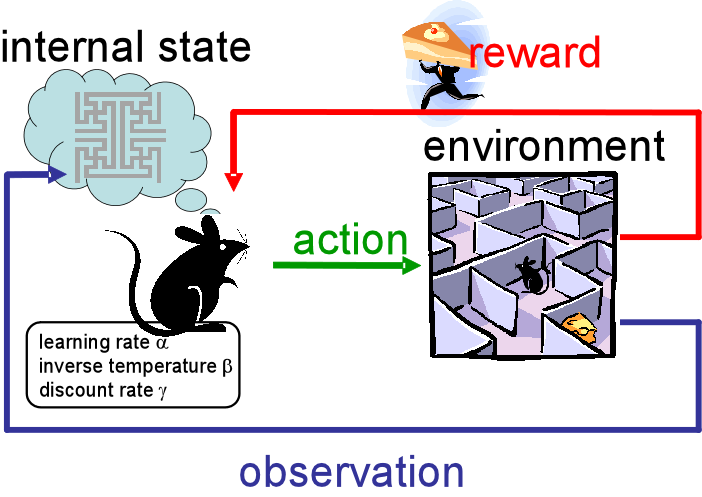
\includegraphics[width=7.5cm]{figures/rl_interaction}
\end{wrapfigure}

\bigskip

\noindent \textbf{Requirements:} Knowledge in Deep Learning, or solid background in Machine Learning. Implementation experience is an advantage. You should be able to read and understand the first 12 chapters of the "Deep Learning Book" by Goodfellow et al. (available for free online from MIT press). If you are interested in the topic but new to deep learning we expect you to complete an introductory deep learning course before applying for the thesis, such as Andrew Ng's coursera course (use the free trial!)\footnote{\url{https://www.coursera.org/specializations/deep-learning}} or this Udacity course\footnote{\url{https://classroom.udacity.com/courses/ud730}}. 
\bigskip

\subsection*{Contacts}
\begin{itemize}
	\item Oliver Richter: \href{mailto:Oliver Richter<richtero@ethz.ch>}{\texttt{richtero@ethz.ch}}, ETZ G63
	\item Gino Brunner: \href{mailto:Gino Brunner <brunnegi@ethz.ch>}{\texttt{brunnegi@ethz.ch}}, ETZ G63
\end{itemize}

% % The part following this line is usually not part of the bait but rather meant as part of the assigmnent for a student when he starts the thesis.
 \newpage
 
\subsection*{Problem statement:}
There are three main frameworks which allows to enforce a hierarchy on a system, namely the option framework , hierarchy of abstract machines (HAM), and the framework of decomposing the Markov decision process (MDP) into smaller MDP's also known as MAXQ decomposition. In this work we concentrate on the option framework. The idea of options is well established since the introduction was relatively long ago, as early as 1999/2000, and hence offers a diverse range of applications and publications.

In this work we want to provide further insight when the introduction of the option framework, which is a significant overhead seen from the perspective of neural networks, is viable for learning tasks in an environments. 

\subsection*{Detailed Project Outline}
We denote the following primary tasks mandatory (on the right side you find a rough estimate for the time that we allocate to the respective task):
\begin{reqlist}
\req Searching the literature for the most relevant topics & \effort{3}
\req New environment definition which allows better tracking of the efficiency of options & \effort{2}
\req Asynchronous actor critic implementation & \effort{2}
\req Option-critic with variable intra option number (adaptive) & \effort{6}
\req Experimenting and improving on the developed architecture & \effort{3}
\req Midterm presentation and report & \effort{5}
\req Option analysis on the constructed environment & \effort{3}
\req Feudal network reconstruction from paper & \effort{5}
\req Testing the Feudal network on our environment & \effort{2}
\end{reqlist}

\subsection*{Extensions}
\noindent Apart from these requirements, we can think of plenty ways to extend our analysis and test hybrid approaches. Of course, you may add your own ideas to this non-exhaustive enumeration:
\begin{itemize}
	\item dynamic feature size (world size)
 	\item hybrid approach of Feudal network and more then one worker
 \end{itemize}

\end{document}
